\begin{frame}{Comparons nos intérêts}
  Avec un(e) partenaire, discute de tes intérêts en faisant des comparaisons.
  Utilise des \emph{pronoms possessifs} autant que possible.
  \begin{columns}
    \column{0.5\textwidth}
      \begin{itemize}
        \small
        \item[] \textbf{Modèle:}
        \item[E1:] Ma musique préférée est la country.
        \item[E2:] \alert{La mienne} est la musique classique. Pourquoi est-ce que tu préfère la country?
      \end{itemize}
      \begin{center}
        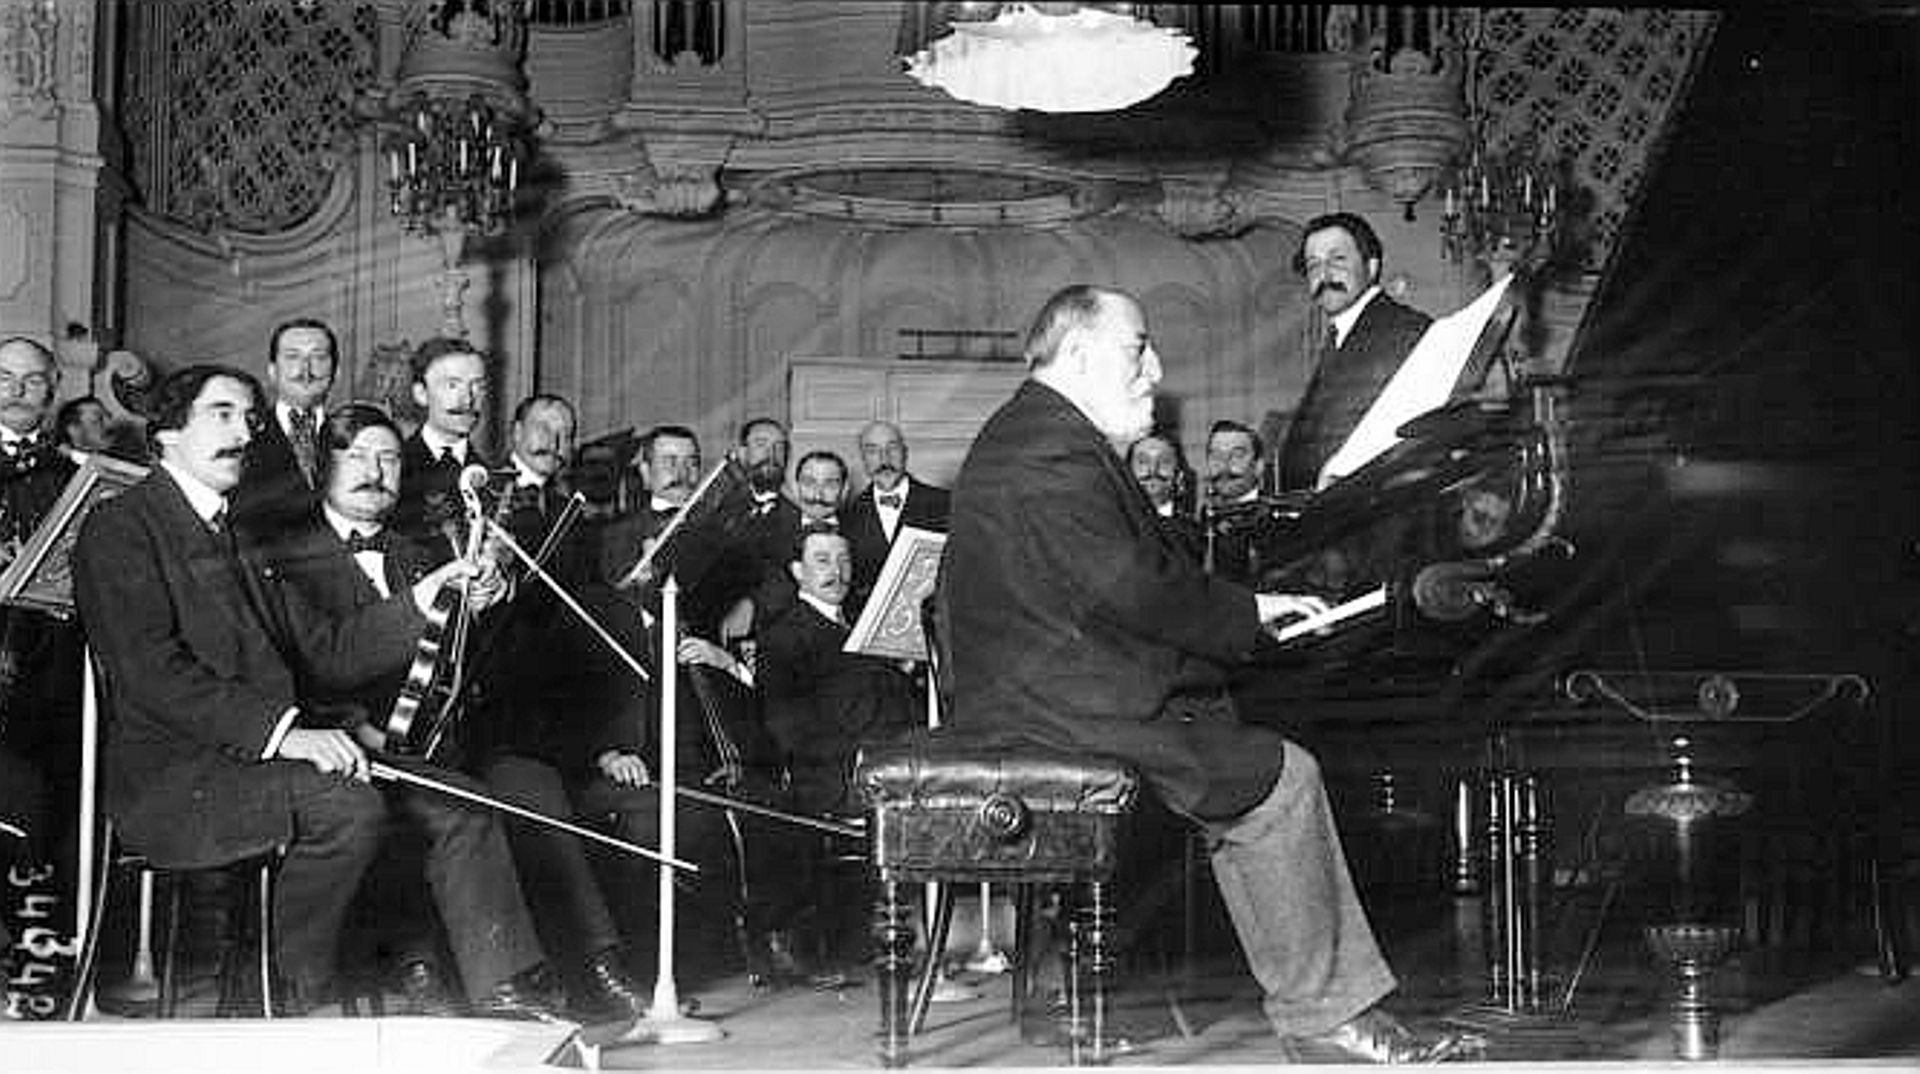
\includegraphics[scale=0.07]{saint-saens.jpg} \\
        {\scriptsize Camille Saint-Saëns en 1913}
      \end{center}
    \column{0.5\textwidth}
      Des sujets possibles:
      \begin{enumerate}
        \item La musique
        \item Les cours
        \item La nourriture
        \item Les films
        \item Les sports
        \item Les activités en plein air
        \item Le théâtre
        \item etc.
      \end{enumerate}
  \end{columns}
\end{frame}